\subsection{Arrays}
\begin{itemize}
	\item An \textbf{array} is a fixed-sized, indexed, homogeneous aggregate type (a collection of items, all of the same type.)
	\item To declare and define an array of four integers:
\begin{lstlisting}[style=C++]
int bar[4];	// Array
int foo; 	// For use later
\end{lstlisting}
	
	\item In the previous code we get a memory environment as follows:
	\begin{center}
		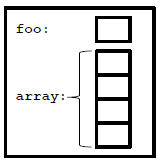
\includegraphics[scale=.9]{sections/lec6/m1.png}
	\end{center}

	\item You can initialize the contents of an array in line:
\begin{lstlisting}[style=C++]
int bar[4] = {1, 2, 3, 4};	// Static Initializer
int foo = 7; 	
\end{lstlisting}
	\item Resulting in the following environment:
	\begin{center}
		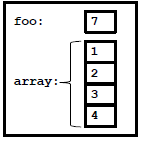
\includegraphics[scale=0.9]{sections/lec6/m2.png}
	\end{center}
\end{itemize}

\subsection{Accessing array elements}
\begin{itemize}
	\item You can access the contents of an array using an ``index''. The index of the first array element is zero, the next is one, and so on.
	\item Each individual element is used just like a regular int, so all of the following are legal:
\begin{lstlisting}[style=C++]
// array = {1, 2, 3, 4}
array[1] = 6;
// array = {1, 6, 3, 4}
++array[1];
// array = {1, 7, 3, 4}
array[0] = array[1];
// array = {7, 7, 3, 4}
\end{lstlisting}
\end{itemize}

\subsection{Passing arrays to functions}
\begin{itemize}
	\item C++ arrays can be passed as arguments to a function.
	\item Suppose we wanted to write a function to add up the contents of an array and we want it to work with any size array.
	\item Here's what the declaration of such a function might look like:
\begin{lstlisting}[style=C++]
int sum(inta[], unsigned int size);
// REQUIRES: there are at least size elements in a[]
// EFFECTS: returns the sum of the first size elements of a[]
\end{lstlisting}

	\item Important things to notice:
	\begin{enumerate}
		\item The declaration of the array argument does not specify the length of the array. That allows the function to work for any length.
		\item \lstinline[style=C++]{sum()} needs to know how long the array actually is (or at least, how many elements to ``sum up''), so the second argument does this.
		\item An unsigned intis used for \lstinline[style=C++]{size} since it can’t be negative. A regular intcould be used, but then the REQUIRES clause would need to catch cases of negative sizes. It’s better to write a complete function.
	\end{enumerate}

	\item Unlike most types we've seen so far, C++ arrays are notpassed by value. They are passed by reference.
	\begin{center}
		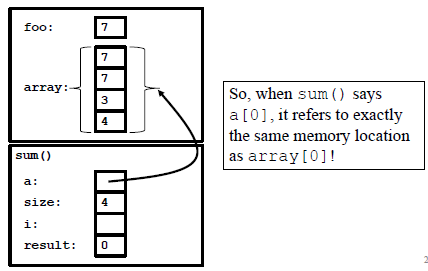
\includegraphics[scale=0.9]{sections/lec6/m3.png}
	\end{center}

	\item The C++ compiler DOES NOT CHECK to make sure that your array reference is legal.
	\item A C-style string is an array of zero or more chars followed by a \lstinline[style=C++]{NULL} character –usually written as \lstinline[style=C++]{\\0}
\begin{lstlisting}[style=C++]
	char a[] = "foo"; // {'f', 'o', 'o' '\0'}
\end{lstlisting}

	\item \textbf{Sentinel}: a special element value for n aggregate type that is:
	\begin{itemize}
		\item Not a legal value for an element of that aggregate 
		\item Signals the ``end'' of the aggregate
	\end{itemize}
\end{itemize}

\subsection{Thinking about memory}
\begin{itemize}
	\item Memory is a linear sequence of storage locations numbered from 0 to a very large number.
	\item Locations that hold some sort of object belonging to the program are \textbf{valid}, others are not.
	\item The location of its object is called its \textbf{address}.
	\item e.g.,
	\begin{center}
		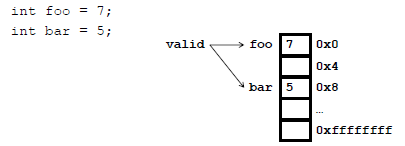
\includegraphics[scale=0.85]{sections/lec6/mem.png}
	\end{center}
\end{itemize}

\subsection{Pointers}
\begin{itemize}
	\item Sometimes we want to explicitly work with the address of anobject. To do this, we use a \textbf{pointer}.
	\item A ``pointer-to-T'' is a variable that can hold the address of some other object of type T.
	\item For example, to declare a pointer to an \lstinline[style=C++]{int}, we would say:
\begin{lstlisting}[style=C++]
int *bar;
\end{lstlisting}

	\item The ``*'' means ``pointer-to''
	\item \lstinline[style=C++]{bar} is a pointer to \lstinline[style=C++]{int}
\begin{lstlisting}[style=C++]
int foo;
int *bar;
bar = &foo;
foo= 1;
\end{lstlisting}
	\item The symbol ``\&'' means ``address-of''. So, this statement says that ``bar is a pointer to an integer, initialized to the address of foo''.
\begin{center}
	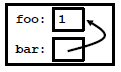
\includegraphics{sections/lec6/ex.png}
\end{center}
\end{itemize}

\subsection{Using pointers}
\begin{itemize}
	\item In addition to setting the value of bar, we can use bar to change the value of the object to which bar points. We do this by saying: \lstinline[style=C++]{*bar = 2;}
	\item The ``*'' here is the ``dereference'' operator
	\item For function pointers the compiler allows us to ignore the ``address-of'' and ``dereference'' operators
\end{itemize}